\documentclass{article}

\usepackage{graphicx}
\usepackage{amsmath,amsfonts,amssymb}
\usepackage[colorlinks,bookmarks,bookmarksnumbered,allcolors=blue]{hyperref}
\usepackage[capitalise]{cleveref}
\usepackage[top=0.75in]{geometry}
\usepackage[dvipsnames]{xcolor}
\usepackage{amsmath} 
\usepackage{esvect}
\usepackage{hyperref}
\usepackage{graphicx}
\usepackage{subcaption}
\usepackage{stfloats}
\usepackage{array}
\usepackage{booktabs}
\usepackage{amsmath}

\begin{document}

\author{Joe Spencer}
\title{Rotor Optimization}
\date{November 23, 2022}
\maketitle

\subsubsection*{Methods}

This report investigates how a rotor's twist and chord length can be adjusted to obtain a rotor that can better fulfill a selected objective function. It is especially desirable to adjust non-dimensional constants like the thrust and torque coefficients to obtain a rotor design that better meets the objective. In this report, the rotor's basic starting profile is kept constant to an APC 10x7 rotor with a NACA 4412 airfoil. Adjusting the chord length of these rotors will make them larger or smaller, but the rotor profile and 4-digit NACA number will remain the same. The objective function for this optimization is shown below in equation 1. \newline

\begin{equation}
\begin{aligned}
	f(x_{1}, x_{2}, x_{3}...) = \eta \\
\end{aligned}
\end{equation} \newline

\noindent The chosen design variables were chord scaling and twist angle. Environmental variables besides these were chosen by estimating reasonable values. Minimum and maximum values for the twist angle and chord were also selected later. The default twist angle bounds chosen were $90^{\circ}$ and $-90^{\circ}$. This way, the entire domain of possible twist angles could be investigated for forward-facing rotors. The chord could be scaled by a maximum factor of up to 2. This would ensure that the optimized propellor's solidity is not different from the original by a factor of more than 2. \newline

\noindent This project uses the SNOW optimizer, developed by the FLOW Lab at BYU, to determine which combination of design variables will be best for a propellor to meet certain requirements defined by the user. The optimizer is confined by several limitations and will stay within 110\% of its original bending moment and 110\% of its original torque, to confine possible designs to the domain of real rotors that could withstand the same loads as the original rotor. \newline

\noindent Chord length and pitching the twist distribution were investigated because these parameters can each be adjusted to affect the shape and performance of the rotor itself. Other parameters, like the rotor's rotational velocity or the wind velocity, for example, will only shift the advance ratio where the rotor is evaluated. \newline

Chord lengths and twist are investigated as design variables because these can both be changed without affecting other aspects of the shape of the rotor itself. scaling all chord lengths by the same amount only scales the entire rotor profile to be magnified without changing anything else about it. This would provide insights into how much solidity is best for a propellor. \newline

\noindent These requirements will demonstrate that the rotor can safely fulfill its design purpose. Other requirements besides these are more flexible and could be modified for future projects depending on an individual rotor's applications. This project's objective function only optimized the chord length and the pitching twist distribution of the rotor. Other parameters used were the rotational velocity, the blade count, the rotor diameter, the hub-to-tip radius, and the free stream velocity. The values for each of these are shown in table 1. \newline

\centering
\title{Table 1: Input Value Limits in Rotor Design \newline}
\title{\emph{These are the default values for each parameter, before the rotor is optimized.}} \label{table:1} \newline
\begin{tabular}{| c | c | c | c |}
	 \hline
  	 \textbf{Parameter} & \textbf{Default Value} & \textbf{Minimum Value} & \textbf{Maximum Value} \\ \hline
	 Chord Length & 100\% length & 50\% & 200\% \\ \hline
	 Twist & $0^{\circ}$ & $-90^{\circ}$ & $90^{\circ}$ \\ \hline
	 Rotational Velocity & \multicolumn{3}{c|}{500 RPM (kept constant)} \\ \hline
	 Blade Count & 2 blades & \multicolumn{2}{c|}{1 to 3 (kept constant)}\\ \hline
	 Hub-to-tip ratio & \multicolumn{3}{c|}{10\% (kept constant)} \\ \hline
	 Air Density & \multicolumn{3}{c|}{1.225 kg/$m^{3}$ (kept constant)} \\ \hline
	 Diameter & \multicolumn{3}{c|}{10 in} \\ \hline
	 Velocity & \multicolumn{3}{c|}{18 m/s (kept constant)} \\ \hline
\end{tabular} \break \newline

\raggedright

Equation 1 describes an optimal propellor that will produce the maximum torque while retaining a high efficiency. This will provide a powerful and efficient propellor. This equation is subjected to constraints to keep it within the domain of real solutions. These constraints are described in equation 2. They say that the total torque, normal moment, and tangential moment each cannot exceed 110\% of those found at the original twist and chord length. \newline

\begin{equation}
\begin{aligned}
	Q_{opt} < 110\% \times Q_{0} \\
	M_{N,opt} < 110\% \times M_{N,0} \\
	M_{T,opt} < 110\% \times M_{T,0} \\
\end{aligned}
\end{equation} \newline

The constraints shown in equation 2 were built into the code as a function argument, so the maximum limit could be raised or lowered as needed. Table 2 shows that these constraints were met by each of the three rotors that were designed, which will be discussed later in this report. \newline

Table 2 shows that for all cases, the optimizer kept the moments and torques experienced by the rotor below their maximum values. This was done in the code by finding the maximum values for the unoptimized rotor, then multiplying these by the safety factor, in this case 110\% or 1.1, and making them into global variables that could be referred to at each step. \newline

\centering
\title{Table 2: Comparison of outputs to limits \newline}
\title{\emph{These values verify that the rotor met maximum moment and torque requirements.}} \label{table:2} \newline
\begin{tabular}{| c | c | c | c |}
	 \hline
  	 \textbf{Propellor} & \textbf{$Q, N \times m$} & \textbf{$M_{N}, N \times m$} & \textbf{$M_{T}, N \times m$} \\ \hline
	 \textbf{Maximum Limit} & 0.040 & $2.971 \times 10^{5}$ & $2.650 \times 10^{4}$ \\
	 \textbf{2 Blades} & 0.003 & $67.864$ & $1171.333$ \\
	 \textbf{3 Blades} & 0.005 & $-670.828$ & $1208.595$ \\
	 \textbf{4 Blades} & 0.006 & $438.019$ & $1314.127$ \\ \hline
\end{tabular} \break \newline

\raggedright
I am searching for the maximum to my objective function, but the optimizer finds a minimum value. I will instead minimuize the reciprocal of the objective function in the optimization. In summary, the optimization will seek to do these things: \newline

\begin{tabular}{l  r}
	 \multicolumn{2}{c}{Table 3: Optimization objective, parameters, and constraints}  \\
  	Minimize: & $\frac{1}{\eta}$ \\ \hline
  	By varying: & scale of the chord, $c$ \\ 
  	 & twist angle, \\  \hline
  	Subject to & total torque less than 110\% of original \\ 
	 & normal moment less than 110\% of original \\ 
	 & tangential moment less than 110\% of original \\ 
	 & $-90^{\circ} <$ twist $< 90^{\circ}$ \\
	 & $50\% <$ chord magnification $< 200\% $
\end{tabular} \newline

\subsubsection*{Results and Discussion}

This research optimized the twist and chord scaling of rotors with 2, 3, and 4 blades, at the conditions described in table 1. The results are displayed in table 4. The optimal values differ from the original values for every rotor tested, by slightly different amounts. Increasing the blade count changed both the optimal chord scaling and twist angle. \newline

The optimal chord length for each rotor appears to be the chord length that is decreased by half, which is the minimum chord length allowed for the analysis. In the \href{https://github.com/JoeSpencer1/497R-Projects/blob/main/Airfoil Analysis/Airfoil_Analysis.pdf}{Airfoil Analysis}, I had found that increasing the chord magnitude increased both the lift and drag coefficients of the airfoil. A propellor with more blades will require less chord length to obtain the same power and torque, but the chord length for maximum efficiency appears to be constant. \newline

\centering
\title{Table 4: Comparison of outputs to limits \newline}
\title{\emph{The optimal chord length and twist angle are shown for different blade counts.}} \label{table:3} \newline
\begin{tabular}{| c | c | c |}
	 \hline
	 \textbf{Blade Count} & \textbf{Chord Scaling} & \textbf{Twist Angle} \\ \hline
	 3, unoptimized & 1.00 & $0^{\circ}$ \\
	 2 & 0.500 & $-11.561^{\circ}$ \\
	 3 & 0.500 & $-11.669^{\circ}$ \\
	 4 & 0.500 & $-11.624^{\circ}$ \\ \hline
\end{tabular} \break \newline

\raggedright
Propellors with 2, 3, and 4 blades each had negative optimal twist angles, close to 11.6 degrees. The rotor with two blades had the optimal twist angle highest in magnitude. Airfoil analysis performed previously has discovered that the lift coefficient is close to zero angles of attack with low magnitude, and that the drag coefficient increases dramatically at negative angles of attack with higher magnitudes for thicker airfoils. Therefore, a rotor with a slight negative twist angle will have low drag and high efficiency. \newline

\begin{figure}
  \centering
  \subfloat[Efficiency]{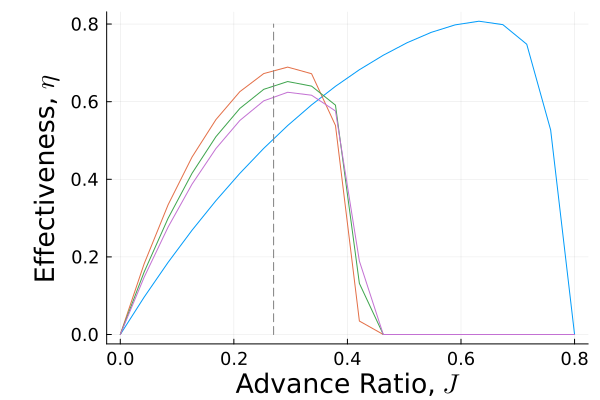
\includegraphics[width = .40\textwidth]{Plots/Figure_1.png}}
  \subfloat[Thrust Coefficient]{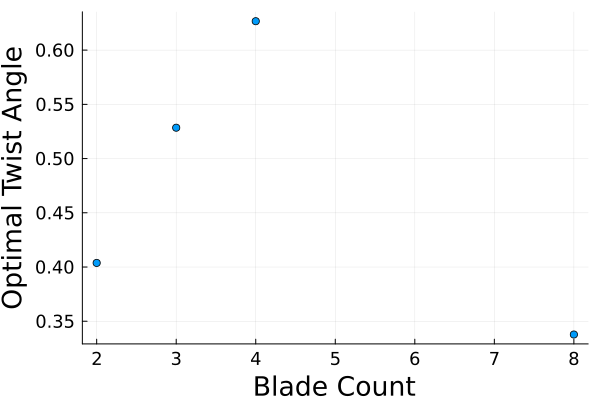
\includegraphics[width = .40\textwidth]{Plots/Figure_2.png}}

  \subfloat[Torque Coefficient]{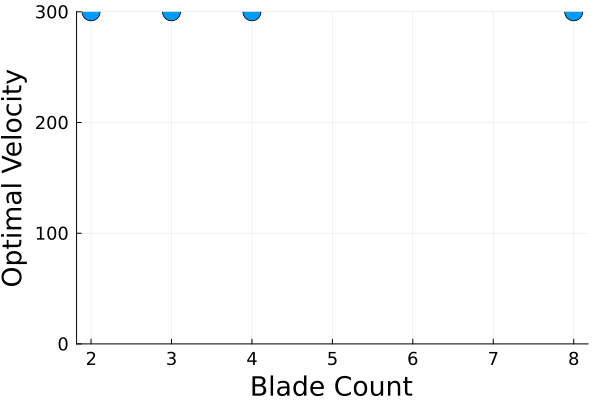
\includegraphics[width = .80\textwidth]{Plots/Figure_3.png}}\hspace{1em}
  \caption{Efficiency, Thrust Coefficients, and Torque Coefficients Compared at Different Advance Ratios}
  \captionsetup{aboveskip=0pt,font=it}
  \caption*{These plots visually represent how optimized rotors are different from the original rotor.}
  \label{fig:1}
\end{figure}

Optimized rotors fulfilled the objective function better than the original rotor did. Figure 1 shows shows that the rotor efficiencies were only optimized at the advance ratio shown with the vertical line. They increased the product of the efficiency, $\eta$, and the thrust coefficient, $C_{T}$, at the advance ratio selected for the optimization, which was found at the 18 m/s free stream velocity, 10 in. outer diameter, and 500 RPM rotational velocity summarized in table 1. After the propellor was optimized at the advance ratio shown below, it was measured at a variety of different advance ratios. \newline \break

\begin{equation}
\begin{aligned}
	J = \frac{v_{a}}{nD} = \frac{v_{a}}{\frac{RPM}{60}D} \\
	J = \frac{18}{\frac{500}{60} \times 20} = 0.27 \\
\end{aligned}
\end{equation} 

Figure 1 shows that the optimized rotors are only optimized for the highest efficiency at an advance ratio $J = 0.27$. At other advance ratios, they are less efficient, and their thrust and torque coefficients are lower across the entire domain of advance ratios. The optimization only found the optimal rotor for the highest efficiency rotor at a specific advance ratio. This rotor would not necessarily fulfill other roles well. \newline

In conclusion, the optimal pitching twist for a rotor to maximize its efficiency is negative for these parameters. The optimal thickness is the minimum possible for propellors of any blade count. \newline

\clearpage

\section{Glossary}

This is a compilation of the previous two glossaries that I have included in my previous \href{https://github.com/JoeSpencer1/497R-Projects/blob/Rotor-Analysis/Airfoil Analysis/Airfoil_Analysis.pdf}{Airfoil Analysis} and \href{https://github.com/JoeSpencer1/497R-Projects/blob/Rotor-Analysis/Rotor Analysis/Rotor_Analysis.pdf}{Rotor Analysis} reports.

\begin{itemize}
	
	\item \hypertarget{J}{Advance Ratio, $J$} - A rotor's advance ratio is a non-dimensional term. It describes the ratio how quickly a rotor is moving relative to the fluid flowing past it. A high advance ratio signifies that either the fluid is moving quickly or the rotor is moving slowly. It is modeled by the following equation, in which $V_{a}$ is the free stream fluid velocity, $n$ is the rotational velocity, and $D$ is the rotor diameter.
	\begin{equation}
	\begin{aligned}
		J = \frac{V_{a}}{n D}
	\end{aligned}
	\end{equation}
		
	\item \hypertarget{alpha}{Angle of Attack, $\alpha$} - The angle of attack, $\alpha$ is the angle between the motion of oncoming fluid and the chord line of the airfoil. a positive $\alpha$ corresponds to a airfoil tilted upwards.
	
	\item \hypertarget{phi}{Angle of Rotation, $\phi$} - The angle of rotation, sometimes denoted by the Greek letter $\phi$, is the angle between the freest stream velocity and the velocity of the airfoil as it rotates. It is used in \hyperlink{BEM}{blade element momentum theory} calculations.

	\item \hypertarget{a}{Axial Induction Factor, $a$} - The axial induction factor is the ratio of the reduction in air velocity at an airfoil to its free stream velocity.
	
	\item \hypertarget{M}{Bending Moment, $M$} - The bending moment a rotor experiences can be modeled by integrating the shear force it is exposed to with respect to its distance in the x-direction. 
	
	\item \hypertarget{BEM}{Blade Element Momentum Theory} - The theory used to calculate local forces on a propellor or wind turbine blade. It employs both \hyperlink{BET}{blade element theory} and \hyperlink{MT}{momentum theory}. These equations are used to recursively find the \hyperlink{a}{axial induction factor, $a$}, \hyperlink{a'}{tangential induction factor}, and \hyperlink{phi}{angle of rotation, $\phi$}
	\begin{equation}
	\begin{aligned}
		\frac{1}{2} W^{2} N c C_{y} = 4 \pi U_{\infty} (1 - a) \times \Omega a' r^{2} \\
		\frac{1}{2} \rho W^{2} N c C_{x} = 4 \pi \rho [(a' \Omega r)^{2} + \Omega^{2}_{\infty} a (1 - a)] r \\
		\sin \phi = \frac{U_{\infty}}{W} (1 - a)
	\end{aligned}
	\end{equation}
In these equations, $a$, $a'$, and $\phi$ are the previously mentioned axial and tangential induction factors and angle of rotation. The airfoil's apparent speed is represented by the letter $W$, $N$ is the number of propellers, $\rho$ is the fluid density, $c$ is the chord length, $C_{x}$ and $C_{y}$ are obtained by the equation below, $U_{\infty}$ is the fluid free velocity, $\Omega$ is the blade's angular speed, and $r$ is the radius to the tip of the blade.
	\begin{equation}
	\begin{aligned}
		C_{x} = c_{l} \cos{\phi} + c_{d} \sin{\phi} \\
		C_{y} = c_{l} \sin{\phi} + c_{d} \cos{\phi}
	\end{aligned}
	\end{equation}
	
	\item \hypertarget{BET}{Blade Element Theory} - Blade element theory calculates the forces on a turbine blade by dividing it into finite pieces and summing the forces on all of these pieces. This theory determines the induced velocity and efficiency of a point along a blade using these equations:
	\begin{equation}
	\begin{aligned}
		v_{i} = \sqrt{\frac{T}{A} \frac{1}{2 \rho}} \\
        		\eta = \frac{\tan{\phi}}{\tan{(\phi + \gamma)}}
	\end{aligned}
	\end{equation}
In these equations, $v_{i}$ is the uniform induced velocity across the disk, $T$ the thrust it experiences, $A$ is its area, $\rho$ is the air density, $\phi$ is the angle to the airfoil's plane of rotation as it moves forward, and $\gamma$ is the difference between $\phi$ and $\beta$, what the airfoil's actual angle of rotation would be if it were stationary.
	
	\item \hypertarget{Camber}{Camber} - An airfoil's camber is represented by the camber line, which runs halfway between its top and bottom surfaces. This line represents the curvature of an airfoil. An airfoil with positive camber is slightly convex on top and slightly concave on its bottom.
	
	\item \hypertarget{c}{Chord, $c$} - An airfoil's chord is the imaginary line running straight from the leading edge of an airfoil to its trailing edge. The chord line is used to find an airfoil's \hyperlink{alpha}{angle of attack}. The chord length distribution shows the length of a rotor's chord at different angular positions around itself. An airfoil with a constant angle of attack $\alpha$ as it generates lift has an elliptic chord distribution.

	\item \hypertarget{CD}{Drag Coefficient (2D), $c_{D}$} - The drag coefficient determines how much drag force opposing motion will be experienced. It comes from a combination of \hyperlink{DP}{pressure drag}, also called form drag, and \hyperlink{VD}{viscous drag} or skin friction. The drag force equation describes it in this way: 
		\begin{equation} \label{eq:13}
		\begin{aligned}
        			D = \frac{1}{2} \rho u^{2} c_{D}
	    	\end{aligned}
		\end{equation}
	
	\item \hypertarget{Vinf}{Freestream Velocity, $V_{\infty}$} - The velocity of an oncoming air flow directly upstream from an airfoil, before it interacts with it.
	
	\item \hypertarget{D/D}{Hub-to-Tip Ratio} - A rotor's hub-to-tip ratio divides the distance along the blade that is actually exposed wind by the entire length of the blade. This needs to be taken into account when calculating constants like the airfoil's \hyperlink{lambda}{tip speed ratio}.
		
	\item \hypertarget{CL}{Lift Coefficient (2D), $c_{L}$} - The lift coefficient is used in the equation below to define how much lift force acts perpendicular to the direction of the oncoming fluid flow.
		\begin{equation} \label{eq:14}
		\begin{aligned}
        			L = \frac{1}{2} \rho u^{2} c_{L}
	    	\end{aligned}
		\end{equation}
	
	\item \hypertarget{LC}{Lift Curve Slope} - The lift curve plots the \hyperlink{CL}{lift coefficient} against the \hyperlink{alpha}{angle of attack} for a single airfoil. This shows the effect that changing the angle of attack will have on the airfoil's total lift force, which can be combined with other airfoils in the case of a wing to find the total lift force experienced by the wing.
		
	\item \hypertarget{M}{Mach Number, $M$} - The mach number is the velocity of an object in proportion to the speed of sound in its medium. When an airfoil is traveling near the speed of sound, its top portions can have fluid velocity above mach 1. When an airfoil is traveling above mach 1, the fluid on both sides of it also have velocities above mach 1 while there are points directly before and after it that are below mach 1.
		\begin{equation} \label{eq:15}
		\begin{aligned}
        			M = \frac{u}{c}
	    	\end{aligned}
		\end{equation}
	
	\item \hypertarget{MT}{Momentum Theory} - Momentum theory defines the power required to produce sufficient thrust to maintain momentum in a blade by the following equation, where $T$ is thrust, $\rho$ is density, $A$ is disc area, and $P$ is power:
	\begin{equation}
	\begin{aligned}
        		P = \sqrt{\frac{T^{3}}{2 \rho A}}
	\end{aligned}
	\end{equation}
		
	\item \hypertarget{NACA}{NACA Airfoil (4-Digit)} - A airfoil shape developed by the National Advisory Committee for Aeronautics (NACA). The first digit is the maximum \hyperlink{Camber}{camber} in tenths of the \hyperlink{c}{chord}. The second digit is the distance in tenths of the maximum camber from the leading edge, out of ten. the final two digits are the maximum airfoil thickness as a percentage of the chord. Descriptions of other NACA numbers can also be found on this \href{https://en.wikipedia.org/wiki/NACA_airfoil}{wikipedia article}. 
		
	\item \hypertarget{CM}{Pitching Moment Coefficient (2D), $c_{M}$} - The moment coefficient is used to calculate the pitching moment a airfoil will experience from its dynamic pressure $q$, area $S$, and chord length $c$.
		\begin{equation} \label{eq:16}
		\begin{aligned}
        			M = q S e c_{M}
	    	\end{aligned}
		\end{equation}

	\item \hypertarget{AP}{Polar} - The airfoil polar is a plot displaying the  \hyperlink{CL}{lift} and  \hyperlink{CD}{drag} coefficients corresponding with each \hyperlink{alpha}{angle of attack} for an airfoil. Examining the ratios of lift to drag is instrumental in choosing the optimal angle of attack.
	
	\item \hypertarget{PFC}{Potential-Flow Code} - A potential-flow code calculates the \hyperlink{CL}{lift}, \hyperlink{CD}{drag}, and \hyperlink{CM}{moment} forces an airfoil experiences at many different points along it. Potential-flow theory assumes constant, incompressible, inviscid fluid flow. It calculates the coefficient for each of these small points and then combines them to find the coefficients along the entire airfoil.
	
	\item \hypertarget{CP}{Power Coefficient, $C_{P}$} - A propellor's coefficient of power signifies how efficient a wind turbine is. It is the ratio of the power generated by a wind turbine to the total power of the wind flowing through it. The power generated or absorbed by an airfoil can be described by the following equation, where $P$ is power, $C_{P}$ is the coefficient of power, $\rho$ is fluid density, $n$ is the velocity in revolutions per second, and $D$ is the propellor diameter. The power coefficient and the \hyperlink{CT}{torque coefficient} are proportional to each other by a factor of $2\pi$.
	\begin{equation}
	\begin{aligned}
		P = \rho n^{3} D^{5} C_{P} \\
		C_{P} = 2 \pi C_{Q}
	\end{aligned}
	\end{equation}
		
	\item \hypertarget{DP}{Pressure Drag} - Pressure drag, also called form drag, comes from the the formation of a vacuum behind an object. The object experiences higher pressure ahead of it than behind it, so the pressure difference pushes it backwards.
	
	\item \hypertarget{APC}{Propellor Identification} - A propellor is identified by 2 numbers, which represent its diameter and its pitch, both in inches. For example, an APC 10x7 propellor is made by Advanced Precision Composites. It has a 10-inch diameter and a 7-inch pitch per revolution.
	
	\item \hypertarget{Re}{Reynolds Number, $Re$} - The Reynolds number is a unit-less number for fluid flow described by the equation below. It can be used to predict patterns in the fluid's flow, using its flow speed $u$, characteristic length $L$, and kinetic viscosity $\nu$, or else by its density $\rho$, flow speed $u$, characteristic length $L$, and fluid density $\mu$.
		\begin{equation} \label{eq:17}
		\begin{aligned}
        			Re = \frac{uL}{\nu} \\
			= \frac{\rho uL}{\mu} 
	    	\end{aligned}
		\end{equation}
	
	\item \hypertarget{sigma}{Rotor Solidity, $\sigma$} - Rotor solidity describes the ratio of a turbine's chord length, $c$, to its spacing, $s$. This is found by the following equation, in which $n_{b}$ is the number of blades, $r_{h}$ is the hub radius, and $r_{t}$ is the tip radius.
	\begin{equation}
	\begin{aligned}
		\sigma = \frac{c}{s} = \frac{c n_{b}}{2 \pi \sqrt{\frac{r^{2}_{h} + r^{2}_{t}}{2}}}
	\end{aligned}
	\end{equation}
	
	\item \hypertarget{ST}{Stall} - Stall occurs when an airfoil's \hyperlink{alpha}{angle of attack} is too great in magnitude, either positive or negative. When the angle of attack is too dramatic, flow separation occurs, reducing rather than augmenting the airfoil's \hyperlink{CL}{lift coefficient} as the angle of attack increases.
	
	\item \hypertarget{a'}{Tangential Induction Factor, $a'$} - The tangential induction factor is the ratio of the increase in air velocity tangential to the airfoil to its free stream velocity.
	
	\item \hypertarget{Th}{Thickness} - An airfoil's thickness can be measured in two different ways, either along its \hyperlink{c}{chord line} or along its \hyperlink{Camber}{camber line}. Thickness measured perpendicular to the camber line is also called the American convention, and thickness measured perpendicular to the chord line is also called the British convention.
	
	\item \hypertarget{CT}{Thrust Coefficient, $C_{T}$} - A rotor's thrust coefficient determines how much thrust in the forward direction an airfoil experiences. Thrust force is directly opposite drag. Please note the similarities and differences between the thrust equation and the \hyperlink{CP}{power equation}.
	\begin{equation}
	\begin{aligned}
		T = \rho n^{2} D^{4} C_{T}
	\end{aligned}
	\end{equation}
	
	\item \hypertarget{lambda}{Tip Speed Ratio, $\lambda$} - A wind turbine's tip speed ratio is the inverse of its \hyperlink{J}{advance ratio, $J$}. It represents the ratio of the speed of the tip of a turbine blade, or $\omega R$, to the wind speed, $v$.
	\begin{equation}
	\begin{aligned}
		\lambda = \frac{\omega R}{v} = \frac{\pi}{J}
	\end{aligned}
	\end{equation}
	
	\item \hypertarget{CQ}{Torque Coefficient, $C_{Q}$} - A rotor's torque coefficient defines how much torque it will experience. A propellor's torque is given by the following equation, in which $Q$ represents torque, $\rho$ is the fluid density, $n$ is the velocity in revolutions per second, $D$ is the diameter, and $C_{Q}$ is the coefficient of torque. The torque coefficient and the \hyperlink{CP}{power coefficient} are proportional to each other by a factor of $2\pi$.
	\begin{equation}
	\begin{aligned}
		Q = \rho n^{2} D^{5} C_{Q} \\
		C_{Q} = \frac{C_{P}}{2 \pi}
	\end{aligned}
	\end{equation}
	
	\item \hypertarget{eta}{Efficiency, $\eta$} - The efficiency of a rotor can be described by the following equation, in which $J$ is the rotor's \hyperlink{J}{advance ratio}, $C_{T}$ is its \hyperlink{CT}{thrust coefficient}, and $C_{P}$ its \hyperlink{CP}{power coefficient}:
	\begin{equation}
	\begin{aligned}
		\eta = J \frac{C_{T}}{C_{P}}
	\end{aligned}
	\end{equation}
	
	\item \hypertarget{T}{Twist Distribution} - Twist distribution along a wing redirects where air flows past it. This causes changes in both the magnitude and location lift and drag forces it experienced as air flows past it.
	
	\item \hypertarget{VD}{Viscous Drag} - Viscous drag, also called skin friction, is drag caused by friction with the fluid particles flowing past an airfoil. Along with \hyperlink{PD}{pressure drag}, it contributes to an airfoil's total \hyperlink{CD}{drag coefficient} airfoil.
	
\end{itemize}

\end{document}